% !TEX root = ../thesis.tex
\chapter{Evaluation} \label{evaluation}
Implementation of our experiment created in Matlab with results explanations enriched with Live script application with dynamic weights setting.
\section{Used software, libraries and predefined functions} \label{subsec:libraries}
\textbf{Matlab 2020a}\\
MATLAB (matrix laboratory) is a fourth-generation high-level programming language and interactive environment for numerical
computation, visualization and programming developed by MathWorks.\\
\\
\textbf{Matlab LiveScript}~\cite{livescript}\\
MATLAB live scripts and live functions are interactive documents that combine MATLAB code with formatted text, equations,
and images in a single environment called the Live Editor.
In addition, live scripts store and display output alongside the code that creates it.\\
Use live scripts and functions to:\\
\begin{itemize}
    \item Visually explore and analyze problems
    \item Share richly formatted, executable narratives
    \item Create interactive lectures for teaching
\end{itemize}\\
\\
\textbf{Matlab Curve Fitting Tool}\\
The Curve Fitting Toolbox provides a collection of GUIs and M-files.
With the toolbox we are able to data preprocessing such as sectioning and smoothing, parametric and nonparametric data fitting,
and also fit statistics which assist us in determining the goodness of fit,analysis capabilities such as extrapolation, differentiation, and integration.
A graphical environment allows you to explore and analyze data sets and fits visually and numerically.\\
\textbf{hhmgenerate}~\cite{hhmgenerate}\\
The function $hmmgenerate$ begins with the model in state 1 at step 0, prior to the first emission.
The model then makes a transition to state $i_1$, with probability $T_{1i_1}$, and generates an emission $a_k_1$ with probability $E_{i_1k_11}$.
$hmmgenerate$ returns $i_1$ as the first entry of states, and $a_k_1$ as the first entry of seq.
$[seq,states] = hmmgenerate(len,TRANS,EMIS)$ takes a known Markov model, specified by transition probability matrix $TRANS$ and emission probability matrix $EMIS$,
and uses it to generate:\\
\begin{itemize}
    \item A random sequence seq of emission symbols
    \item A random sequence states of states
\end{itemize}
The length of both $seq$ and $states$ is $len$.
$TRANS(i,j)$ is the probability of transition from state $i$ to state $j$.
$EMIS(k,l)$ is the probability that symbol $l$ is emitted from state $k$.\\
\\
\textbf{hhmviterbi}~\cite{hhmviterbi}\\
The function $hmmviterbi$ begins with the model in state 1 at step 0, prior to the first emission.
hmmviterbi computes the most likely path based on the fact that the model begins in state 1.
$STATES = hmmviterbi(seq,TRANS,EMIS)$ given a $sequence, seq$, calculates the most likely path through the hidden Markov model
specified by transition probability matrix, $TRANS$, and emission probability matrix $EMIS$. $TRANS(i,j)$ is the probability of transition from state $i$ to state $j$.
$EMIS(i,k)$ is the probability that symbol $k$ is emitted from state $i$.\\
\\
\textbf{shopycrm.com}\\
Online CRM application focused on e-commerce stores which provides all store workflows and get precalculated data which
we will use for our models to simplify the prediction calculation.
\section{Fitting models and prediction} \label{fitting}
Let use Matlab Curve fitting tool to solve our linear and polynomial models as you can see on figure~\ref{cftool},
this predefined tool calculate coefficient for and then the prediction in Matlab Live script was done as we see on figure~\ref{predict}.
These two models was fitted on income data from years 2018 and 2019 as is described in our Experiment (see section~\ref{experiment}).
\begin{figure}[h!]
    \begin{center}
        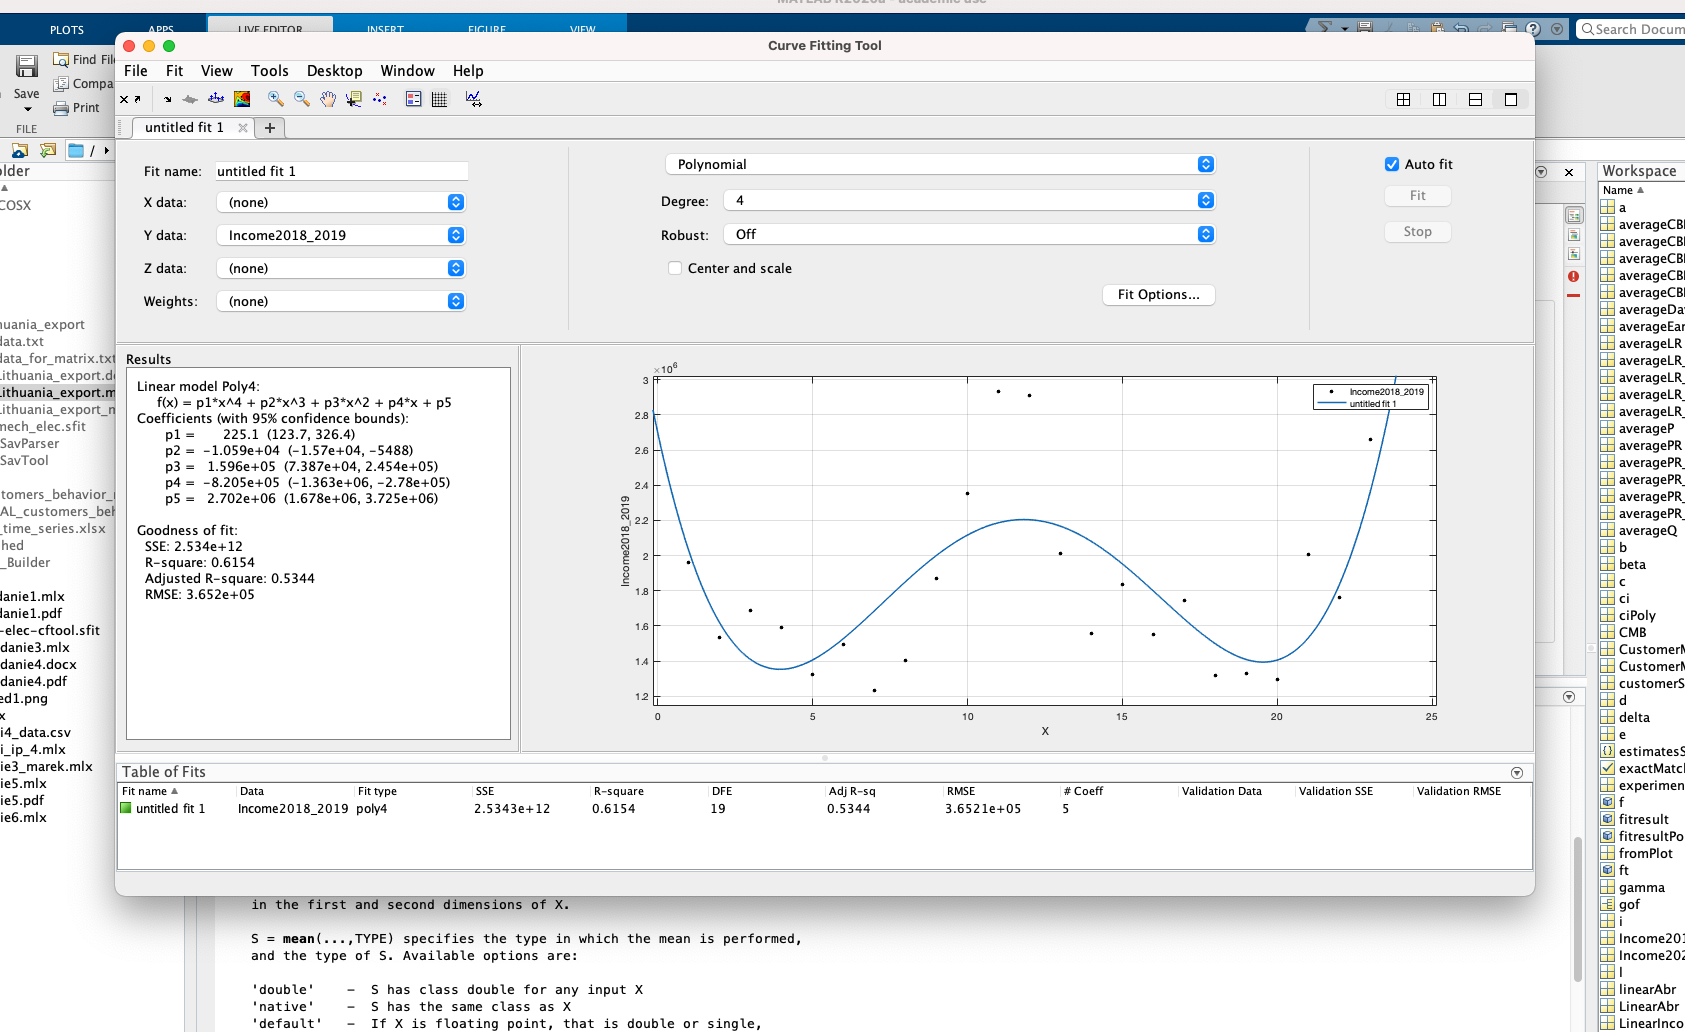
\includegraphics[width=100mm]{cftool.png}
    \end{center}
    \caption{Fitting the data with cftool~\cite{luarn}}
    \label{cftool}
\end{figure}\\
Then Matlab's function $predint$ was used to return income prediction results for year 2020 used fitted linear model.
Polynomial model used other approach to calculate aberration for each month from plotted results as it seen on figure~\ref{predict}.
\begin{figure}[h!]
    \begin{center}
        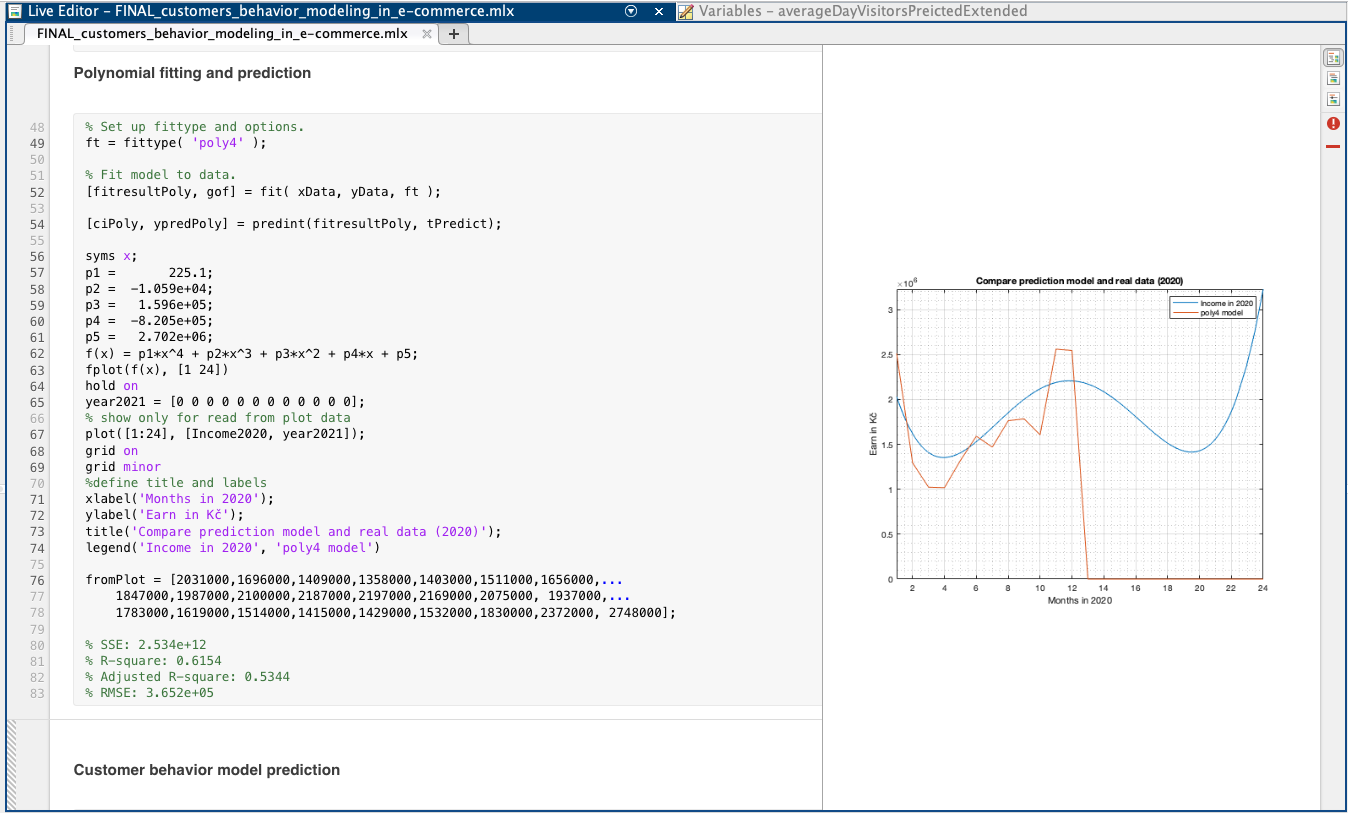
\includegraphics[width=100mm]{predict.png}
    \end{center}
    \caption{Predict income data in live script~\cite{luarn}}
    \label{predict}
\end{figure}\\
Fitted and prepared models from section~\ref{subsec:calculate_models} was compared with real data from year 2020.
On the figure~\ref{plot} is graphical presentation of data and our linear and polynomial models.
It turned out that the first linear model (blue line), is not directly corresponding the data, but it is copying the trend of the income (red line),
polynomial model (green line) returns better results that previous one.
The best results returned from Customer behavior HMM (violet line).
what we should see on figure~\ref{plot} with predicted data to 2020.
\begin{figure}[h!]
    \begin{center}
        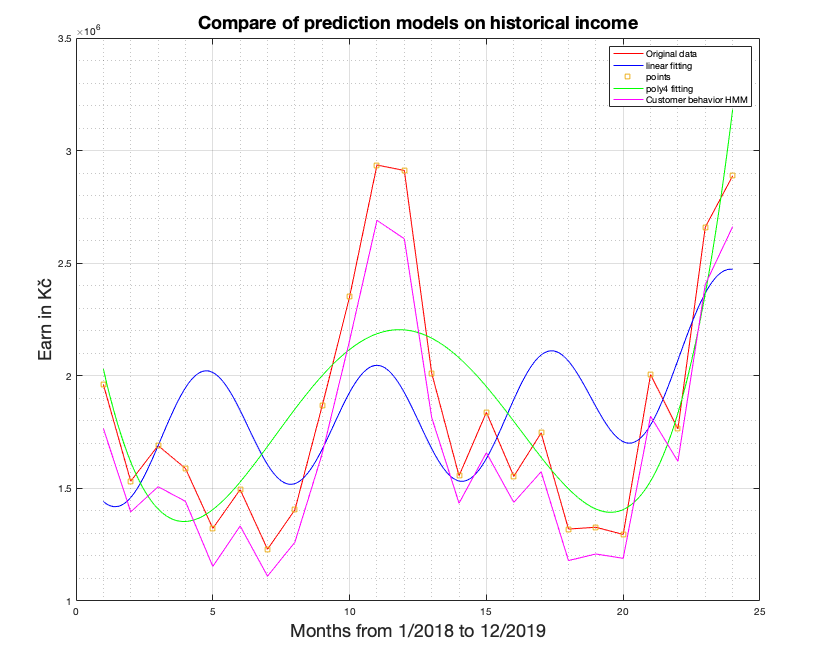
\includegraphics[width=140mm]{plot.png}
    \end{center}
    \caption{Fitting the model on real income from 2018 and 2018}
    \label{plot}
\end{figure}\\
Prediction from Customer behavior HMM was made 10 times.
The final result is arithmetic mean from this prediction which is ten times run to random deviation  was minimised.
Our prediction script is finally written in Matlab Live script with predefined constants based on Megaplay s.r.o data,
but for modeling and dynamic prediction are used Live scripts Controls so in the script we are able to easily set all
constant to model for simulate different situations.
Let see the dynamic function of our prepared model on figure~\ref{app}.
\begin{figure}[h!]
    \begin{center}
        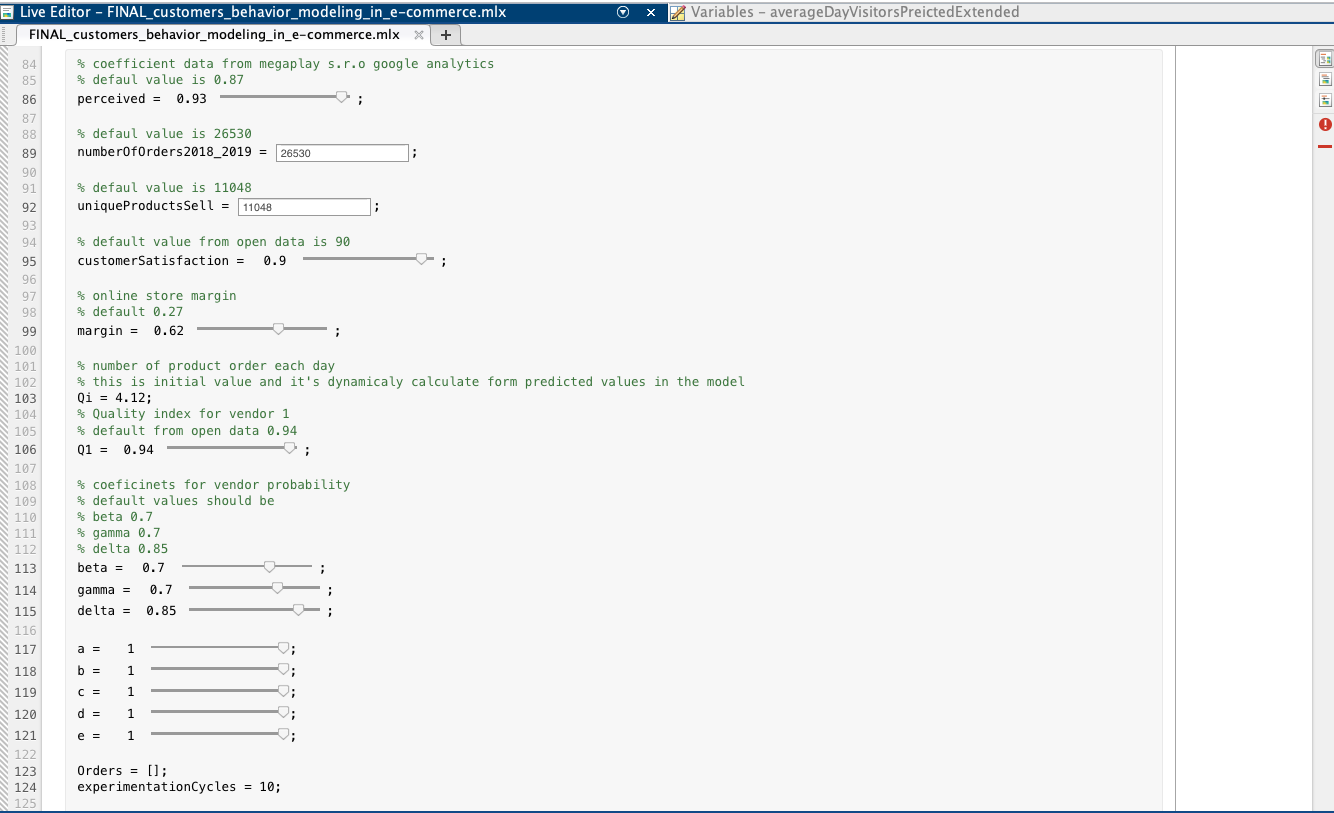
\includegraphics[width=100mm]{app.png}
    \end{center}
    \caption{Live Script application to dynamically set weights and constants for model}
    \label{app}
\end{figure}\\
This precalculated data entered calculation loop.
Next loop read the value of predefined number of customers in each period and simulated the virtual customer behavior in order process.
This feature gives us ability to easily simulate our model in a different situation.
Let see some modeled situation in appendix C section~\ref{apendixc}.
That results are described in the final summary~\ref{summary} same as results from previous regresion models.
\section{Results} \label{compareresults}
On the figure~\ref{results} prediction results are seen.
For the year 2021 is compared with the real income and we can see that the polynomial and Customer behavior HMM model
get good results, in the opposite of that results linear model predict the trend of the income.

\begin{figure}[h!]
    \begin{center}
        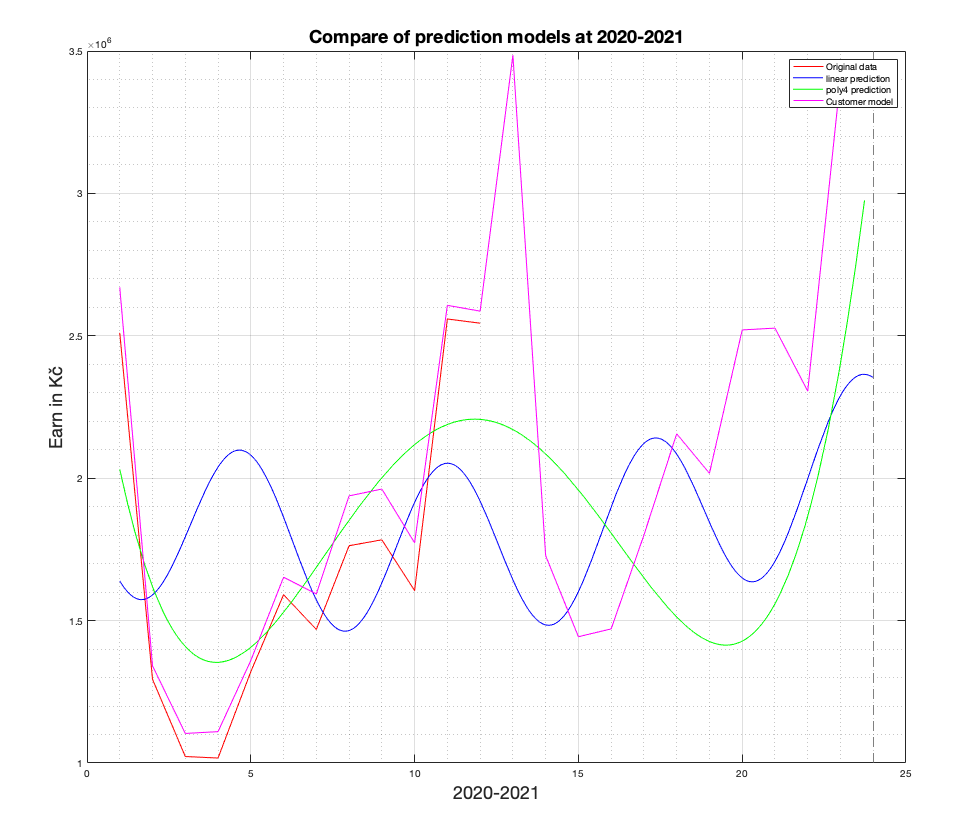
\includegraphics[width=140mm]{results.png}
    \end{center}
    \caption{Prediction from models for years 2020-2021, with real income for 2020.}
    \label{results}
\end{figure}\\
In the graphical view we saw that all our models copy the income, but some of them are easier to calculate, this differences you can see described in Summary (see section~\ref{summary}).
Get the experiment methodology (see section~\ref{subsec:result_metodology}) to models compare table created.
As it see in the table~\ref{compare} out Customer behavior HMM return best results from all tested models.
\begin{table}[h!]
    \begin{center}
        \begin{tabular}{ | l | c | c | c |}
            \hline
            & \textbf{}$ \textbf{linear model} & \textbf{polynomial model} & \textbf{Customer behavior HMM}\\
            \hline
            \textbf{SSE} & 5,165.10^{12} & 2,534.10^{12} & 1,583.10^{11} \\
            \textbf{R-square} & 0,2162 & 0,6154 & 0,95 \\
            \textbf{RMSE} & 4,959.10^5 & 3,652.10^5 & 1,149.10^5\\
            \hline
        \end{tabular}
    \end{center}
    \caption{Compare fit of goodness for models.}
    \label{compare}
\end{table}\\
On the table~\ref{Compare results} are calculated percent aberration from real income in the year 2021.
We saw the first month linear model reached the best results, but in next months is the best results served by Customer behavior HMM.
\begin{table}[h!]
    \begin{center}
        \begin{tabular}{ | l | c | c | c |}
            \hline
            {\textbf{Month}} & \textbf{Linear model} & \textbf{Polynomial model} & \textbf{Customer behavior HMM}\\
            \hline
            1/2021 & 6 & 24 &  7\\
            2/2021 & 74 & 31 & 6\\
            3/2021 & 129 & 38 & 7\\
            4/2021 & 163 & 38 & 13\\
            5/2021 & 134 & 6 & 4\\
            6/2021 & 111 & 5 & 3\\
            7/2021 & 132 & 13 & 7\\
            8/2021 & 92 & 5 & 11\\
            9/2021 & 98 & 11 & 9\\
            10/2021 & 144 & 31 & 10\\
            11/2021 & 75 & 17 & 2\\
            12/2021 & 94 & 16 & 3\\
            \hline
        \end{tabular}
    \end{center}
    \caption{Compare aberration (\%) from real income 2020}
    \label{Compare results}
\end{table}\\
Calculated result per each quarter in 2020 can bee seen at the table~\ref{qResults} is showing to us the oscillation of prediction.
\begin{table}[h!]
    \begin{center}
        \begin{tabular}{ | l | c | c | c |}
            \hline
            & \textbf{Linear model} & \textbf{Polynomial model} & \textbf{Customer behavior HMM}\\
            \hline
            1Q (\%) & 69,66 & 30,81 & 6,42\\
            2Q (\%) & 135,83 & 15,00 & 6,50\\
            3Q (\%) & 107,41 & 9,64 & 9,25\\
            4Q (\%) & 104,25 & 21,21 & 4,89\\
            \hline
        \end{tabular}
    \end{center}
    \caption{Quarterly results}
    \label{qResults}
\end{table}
\newpage
